% !TeX root = ../main.tex
\documentclass[../main.tex]{subfiles}
\begin{document}
\chapter{cmake学习}
CMake是个一个开源的跨平台自动化建构系统,并不依赖于某特定编译器,并可支持多层目录、多个应用程序与多个库的编译。 它用配置文件控制建构过程(build process)的方式和Unix的make相似,只是CMake的配置文件取名为CMakeLists.txt。CMake并不直接建构出最终的软件,而是产生标准的工程(如Unix的Makefile或Windows Visual C++的projects)。这使得熟悉某个集成开发环境(IDE)的开发者可以用标准的方式生成对应的工程,并进行编译侯建。 CMake配置文件(CMakeLists.txt)可设置源代码或目标程序库的路径、产生适配器(wrapper)、还可以用任意的顺序建构可执行文件。CMake支持in-place构建(生产的工程和源代码在同一个目录树中)和out-of-place构建(生成的工程文件与源代码不在同一个文件夹下),因此可以很容易从同一个源代码目录树中编译出多个二进制文件。CMake也支持静态与动态程序库的编译。
\section{cmake概述}
“CMake”这个名字是"Cross platform Make"的缩写。虽然名字中含有"make",但是CMake和Unix上常见的“make”系统是分开的,而且更为高端。 它可与原生建置环境结合使用,例如:make、苹果的Xcode与微软的Visual Studio。因此使用cmake进行工程管理具有如下优势:
\begin{enumerate}
    \item 跨平台使用。cmake支持目前市面上几乎多有的操作系统,便于进行工程移植。
    \item 不依赖于编译器。cmake生成工程时,可以根据当前的平台选择合适的编译器和工具链,并能方便的找到工程中的依赖库。
\end{enumerate}
\section{cmake安装}
\subsection{Windows安装}
windows下直接下载二进制安装包进行安装即可,安装以后需要设置环境变量,将cmake.exe所在的路径添加到环境变量PATH中,如图所示:
\begin{figure}[H] % 当前位置插入图像
    \centering
    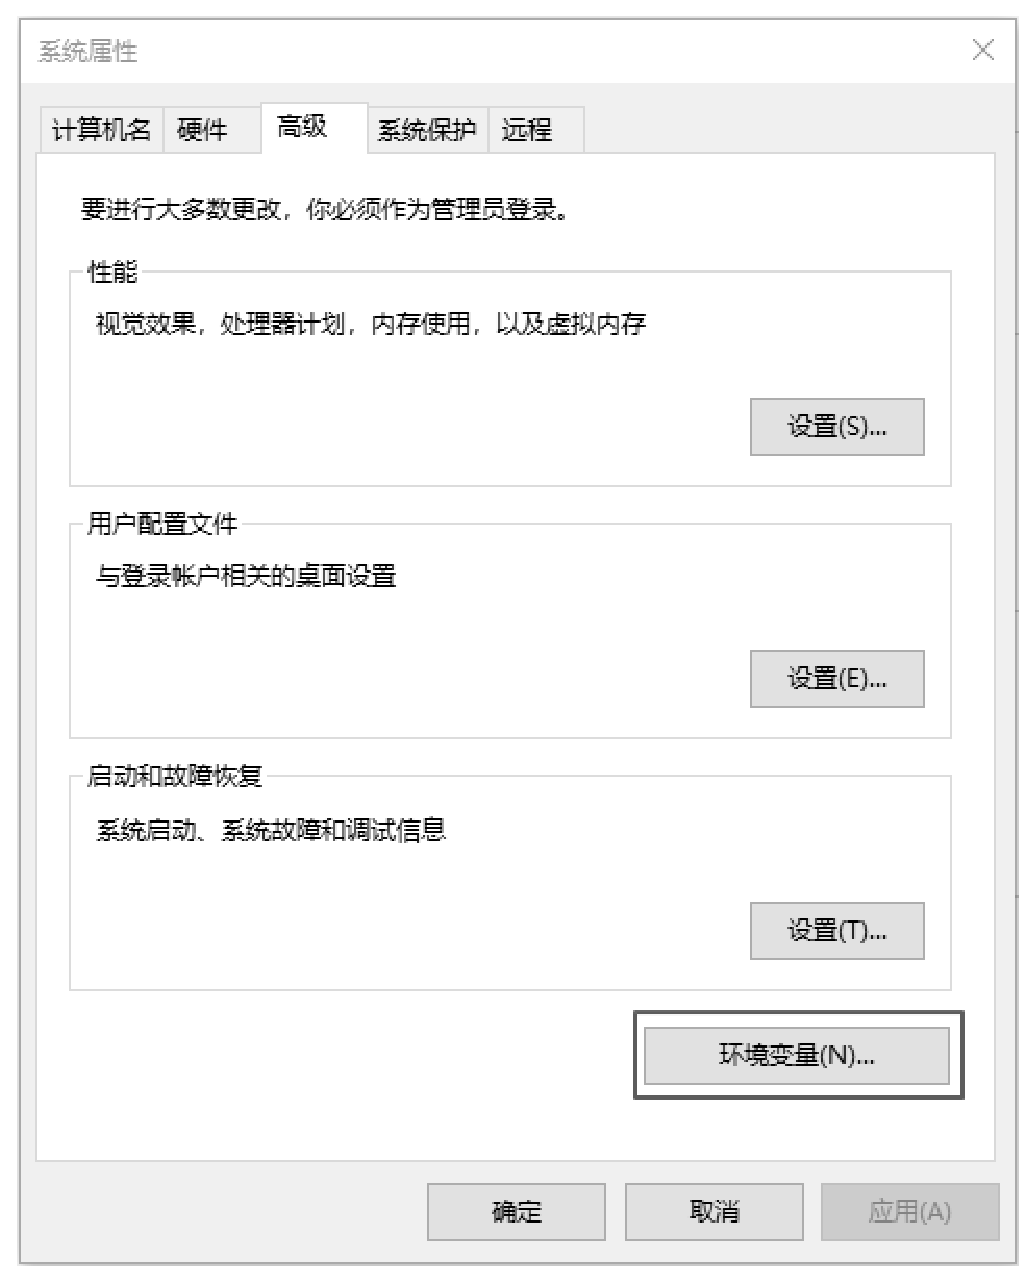
\includegraphics[width=0.5\textwidth]{set_env.eps}
    \caption{设置环境变量}
    \label{设置环境变量}
\end{figure}
\subsection{Linux安装}
linux安装使用Linux发行版自带的包管理器安装即可,Ubuntu的命令行安装如下:
\begin{lstlisting}[caption={Linux安装Cmake}]
    sudo apt install cmake
\end{lstlisting}
\section{cmake入门}

\end{document}